\section{Energieeichung}
\label{section:Energieeichung}

Um eine Aussage über die Energie der von den Präparaten emittierten Strahlung zu machen, muss erstmal ein Zusammenhang zwischen 
den Kanalnummern des Vierkanalanalysators und den Energiewerte hergestellt werden. Wir nehmen dazu an, dass der Zusammenhang linear sei. Nun bringen wir 
die charakteristischen Linien dreier Präparate – siehe Abbildung \ref{bild:Energieeichung} – mit Kanalnummern in Verbindung. Danach bestimmen 
wir via linearer Regression die Parameter $E_0$  für den y-Achsenabschnitt und $m$ für die Steigung.\\

\begin{figure}[h]
    \centering
    \captionsetup{justification=centering,margin=1cm}
    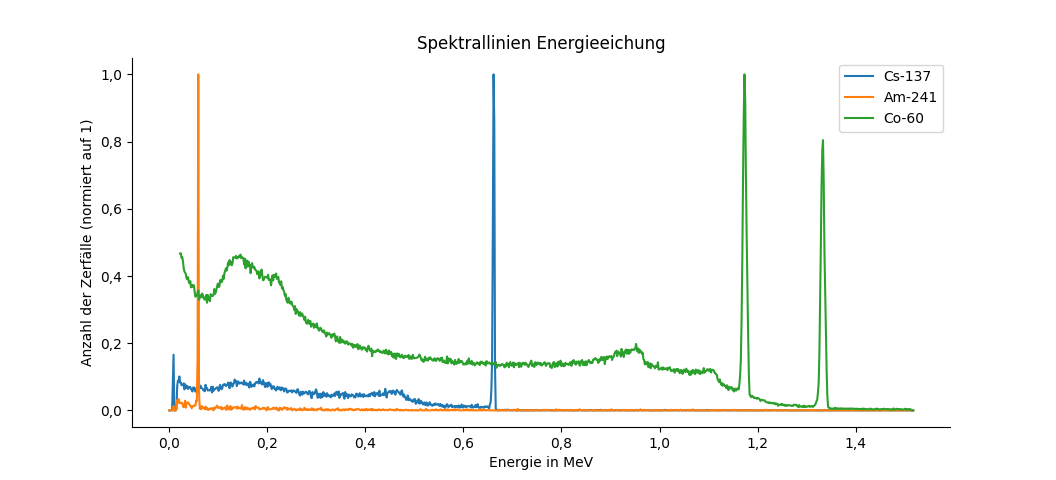
\includegraphics[width = \linewidth]{Bilder/Auswertung/EnergieeichungLinien.png}
    \caption{Spektren von Co-60, Cs-137 und Am-241 im Bereich 0-1,4\,MeV nach Energieeichung. Die Linien sind sehr schmal, was sie gut für die Eichung macht.}
    \label{bild:EichungDrei}
\end{figure}




Die drei verwendeten Präparate/Emissionslinien  sind in Tabelle \ref{Eichung} dargestellt.
 \begin{table}[h]
    \centering
     \begin{tabular}{lcr}
        Isotop & Energie (MeV) & Kanalnummer \\
        \toprule
         Cs-137 & 0,6616  & 447\\
         Am-241 & 0,0594 & 41\\
         Co-60 & 1,1732 & 792\\
     \end{tabular}
     \caption{Zur Energieeichung verwendete Spektrallinien}
     \label{Eichung}
 \end{table}

 Die Peaks wurden hier einfach abgelesen, da diese beim Gammaspektrum so schmal sind, dass eindeutig feststellbar ist, in welchem Kanal der Peak liegt.
 Mit linearer Regression erhält man $E_0 = -1386.75067405 \mathrm{ eV}$ und $m = 1483.09394689 \frac{\mathrm{eV}}{\mathrm{Kanal}}$.
 Dabei sieht man sehr gut an Grafik \ref{Eichgerade}, dass die Annahme eines linearen Zusammenhangs gerechtfertigt ist und der Vierkanalanalysators in 
 diesem Bereich linear arbeitet.

 \begin{figure}[ht]
    \captionsetup{justification=centering,margin=1cm}
     \centering
     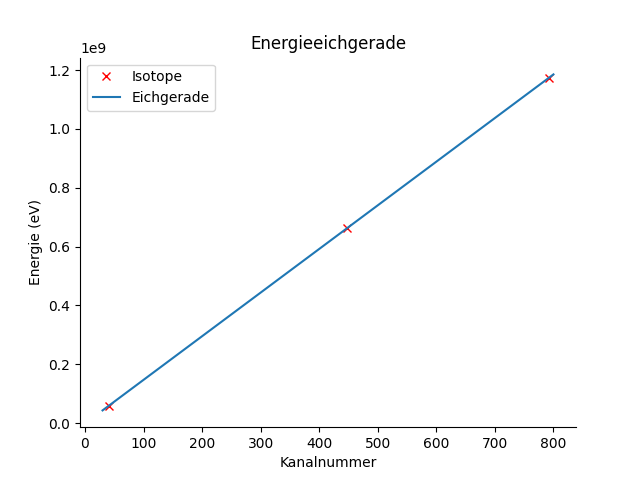
\includegraphics[width = \linewidth]{Bilder/Auswertung/EnergieeichgeradeGamma.png}
     \caption{Eichgerade anhand der oben verwendeten Isotope. Die Fehler sind zu klein um sie in dieser Grafik zu sehen}
     \label{Eichgerade}
 \end{figure}